\section{Results and Discussion}
\label{sec:results}
\subsection{Positive timing benefit does not cover the cost of acting}
The main result is a separation between gross timing information and its value after changing the schedule. Under the primary hypothetical cost specification, full exposure to the learned profile generates average price alignment of $0.00370$ basis points. Its additional curvature cost is $0.00805$ basis points, while the baseline-gradient term is zero to numerical precision. The resulting average objective gain is $-0.00436$ basis points, with a conditional 95\% interval of $[-0.00829,-0.00047]$. The forecast-induced reallocation aligns positively with subsequent price changes on average, but that benefit does not cover the model's charge for departing from the baseline.

\begin{table}[htbp]
\centering\small
\caption{Matched endpoint forecasts and primary execution outcomes. All quantities are basis points under $\eta=2,r=1$. Price alignment and curvature are the terms in the gain decomposition; intervals are conditional day-bootstrap summaries. Parallel gains are analytically zero, with raw absolute mean numerical residuals below $1.5\times10^{-14}$.}
\label{tab:profiles}
\resizebox{\linewidth}{!}{\begin{tabular}{lrrr}
\toprule
Profile & Price alignment & Curvature & Net gain [95\% interval] \\
\midrule
Parallel & 0.00000 & 0.00000 & 0.00000 [0.00000, 0.00000] \\
Learned & 0.00370 & 0.00805 & -0.00436 [-0.00829, -0.00047] \\
Ramp & 0.00339 & 0.00434 & -0.00095 [-0.00520, 0.00285] \\
Mirror & -0.00370 & 0.00805 & -0.01175 [-0.01537, -0.00832] \\
\bottomrule
\end{tabular}
}
\end{table}

\begin{figure}[htbp]\centering
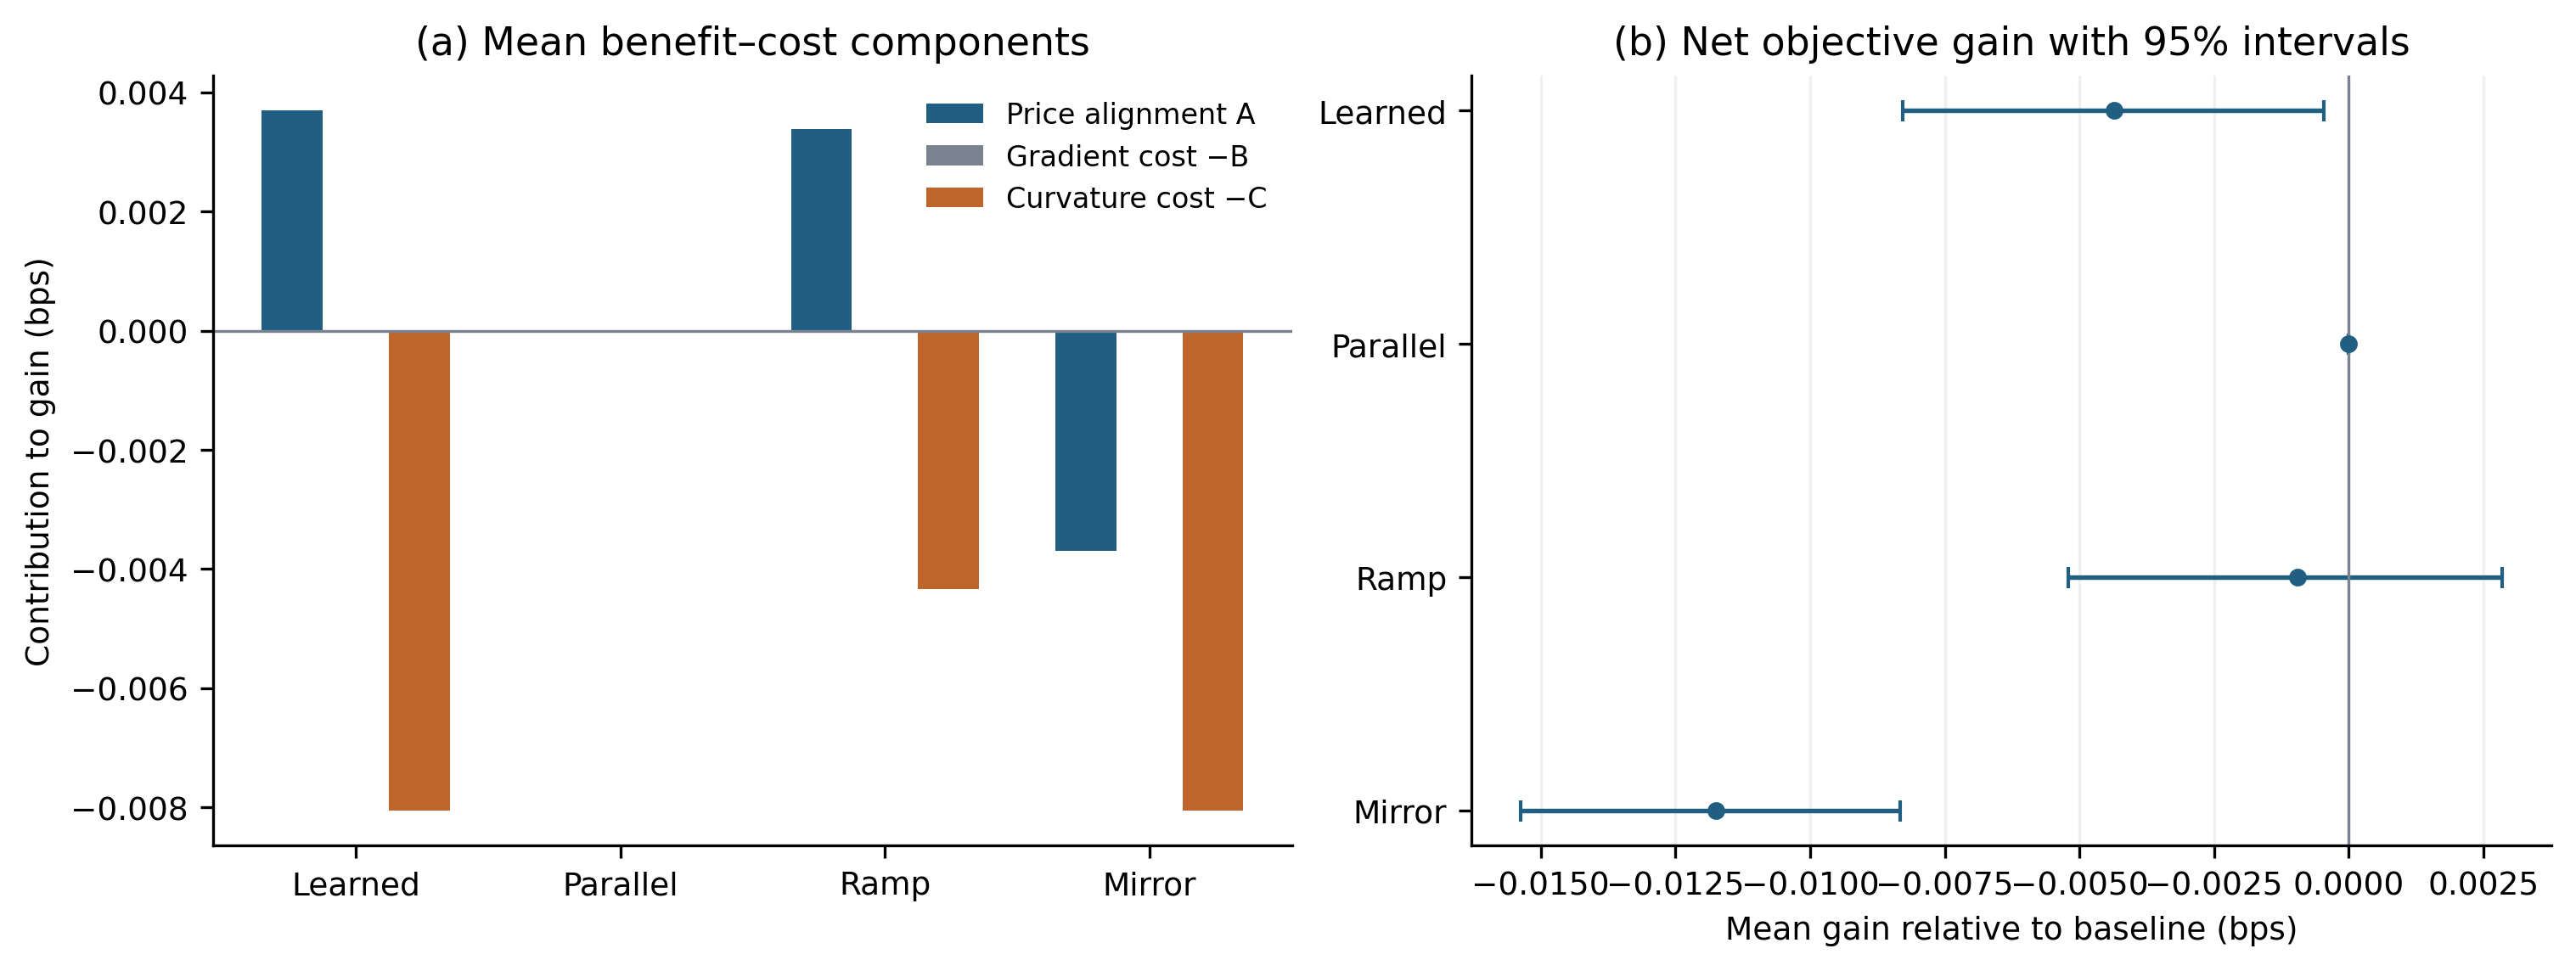
\includegraphics[width=\linewidth]{figures/fig03_benefit_cost.png}
\caption{Primary benefit--cost decomposition and matched-profile gains. Panel (a) reports episode-weighted $A$, $-B$ and $-C$, which sum to objective gain; $B$ is numerically zero. Panel (b) shows conditional 95\% calendar-day bootstrap intervals, resampling both assets jointly. The mirror is a diagnostic counterfactual.}
\label{fig:benefitcost}
\end{figure}

Figure~\ref{fig:benefitcost} displays this decomposition alongside the net outcomes. The first-order baseline term vanishes because the primary baseline lies in the interior of the nonnegative simplex. Its cost gradient is therefore constant across coordinates and orthogonal to feasible schedule changes. The remaining comparison has a direct economic meaning: the positive linear price benefit competes with a quadratic cost of shifting the order. Average shifted quantity is approximately $1.82\%$ of the parent order. Even this relatively small reallocation can be excessive when predictive timing information is weak.

The magnitude matters as well as the sign. The full-exposure loss is approximately $0.44$ parts per million of reference notional within the assumed objective. It would be misleading to turn this statistically distinguishable model difference into a claim of commercially material losses. The evidence supports a diagnostic distinction---positive timing alignment is insufficient for beneficial execution---at a small model-based scale.

\subsection{Identical endpoint scores conceal different schedule outcomes}
Table~\ref{tab:profiles} holds every terminal forecast fixed while changing the within-horizon profile. The parallel profile reproduces the baseline, as required by price-level invariance. The ramp has mean gain $-0.00095$ basis points, with interval $[-0.00520,0.00285]$. The mirror has mean gain $-0.01175$ basis points, with interval $[-0.01537,-0.00832]$. These differences cannot be attributed to changes in endpoint root-mean-square error, hit rate or $R^2$: those predictions and scores are identical by construction.

For the primary specification, the learned and mirrored schedules incur the same average curvature cost, approximately $0.00805$ basis points. Their price-alignment terms have opposite signs, approximately $0.00370$ and $-0.00370$. Reversing temporal contrasts therefore reverses gross timing benefit while retaining the same endpoint prediction. The ramp induces a smaller curvature cost, approximately $0.00434$ basis points, against price alignment of $0.00339$. Its smaller net loss illustrates that a less expensive response can outperform a more detailed estimated path without improving terminal accuracy.

The paired learned-minus-ramp difference is $-0.00341$ basis points, interval $[-0.00770,0.00101]$. The learned profile is consequently not demonstrably superior to this restricted construction. Its learned-minus-mirror difference is $0.00739$ basis points, interval $[0.00076,0.01468]$. The latter result verifies the importance of temporal orientation in this replay, but is not a competitive forecasting victory: the mirror was designed to reverse that orientation. The diagnostic's contribution rests on exposing an omission in endpoint evaluation, rather than on choosing a winning profile.

\subsection{Window heterogeneity and weak endpoint predictability}
Table~\ref{tab:windows} reports all twelve asset--month windows. Terminal hit rates range from $47.9\%$ to $52.6\%$, and terminal $R^2$ values remain close to zero. The simple imbalance specification thus provides limited endpoint predictive evidence in this sample. Full learned exposure produces positive objective gains in five windows and negative gains in seven. The pooled negative result is not a statement that every month or both assets at every date behave identically.

\begin{table}[htbp]
\centering\small
\caption{All primary evaluation windows. Gains are objective basis points; $w_P$ and $w_C$ are fitted on the preceding month. Terminal diagnostics apply identically to all matched profiles. All dates are in 2026.}
\label{tab:windows}
\resizebox{\linewidth}{!}{\begin{tabular}{llrrrrrr}
\toprule
Asset & Month & Hit rate & Terminal $R^2$ & Learned & Ramp & $w_P$ & $w_C$ \\
\midrule
BTC & 03 & 51.9\% & -0.00005 & 0.00184 & 0.00024 & 0.000 & 0.000 \\
BTC & 04 & 49.0\% & -0.00452 & -0.03025 & -0.01944 & 0.000 & 0.000 \\
BTC & 05 & 52.6\% & -0.00037 & -0.00648 & -0.00086 & 0.058 & 0.000 \\
BTC & 06 & 48.8\% & -0.00022 & 0.00003 & 0.00168 & 0.000 & 0.000 \\
BTC & 07 & 50.0\% & 0.00007 & -0.00035 & 0.00001 & 0.520 & 0.000 \\
BTC & 08 & 49.5\% & -0.00127 & 0.00488 & -0.00889 & 0.000 & 0.000 \\
ETH & 03 & 50.5\% & -0.00046 & -0.00535 & -0.00224 & 0.000 & 0.000 \\
ETH & 04 & 47.9\% & -0.00006 & -0.02624 & -0.00140 & 0.049 & 0.000 \\
ETH & 05 & 50.5\% & 0.00034 & -0.00809 & 0.00434 & 0.000 & 0.000 \\
ETH & 06 & 48.4\% & -0.00002 & -0.00072 & 0.00273 & 0.620 & 0.000 \\
ETH & 07 & 51.1\% & 0.00189 & 0.00695 & 0.00692 & 0.824 & 0.000 \\
ETH & 08 & 50.7\% & 0.00070 & 0.01023 & 0.00508 & 0.674 & 0.000 \\
\bottomrule
\end{tabular}
}
\end{table}

\begin{figure}[htbp]\centering
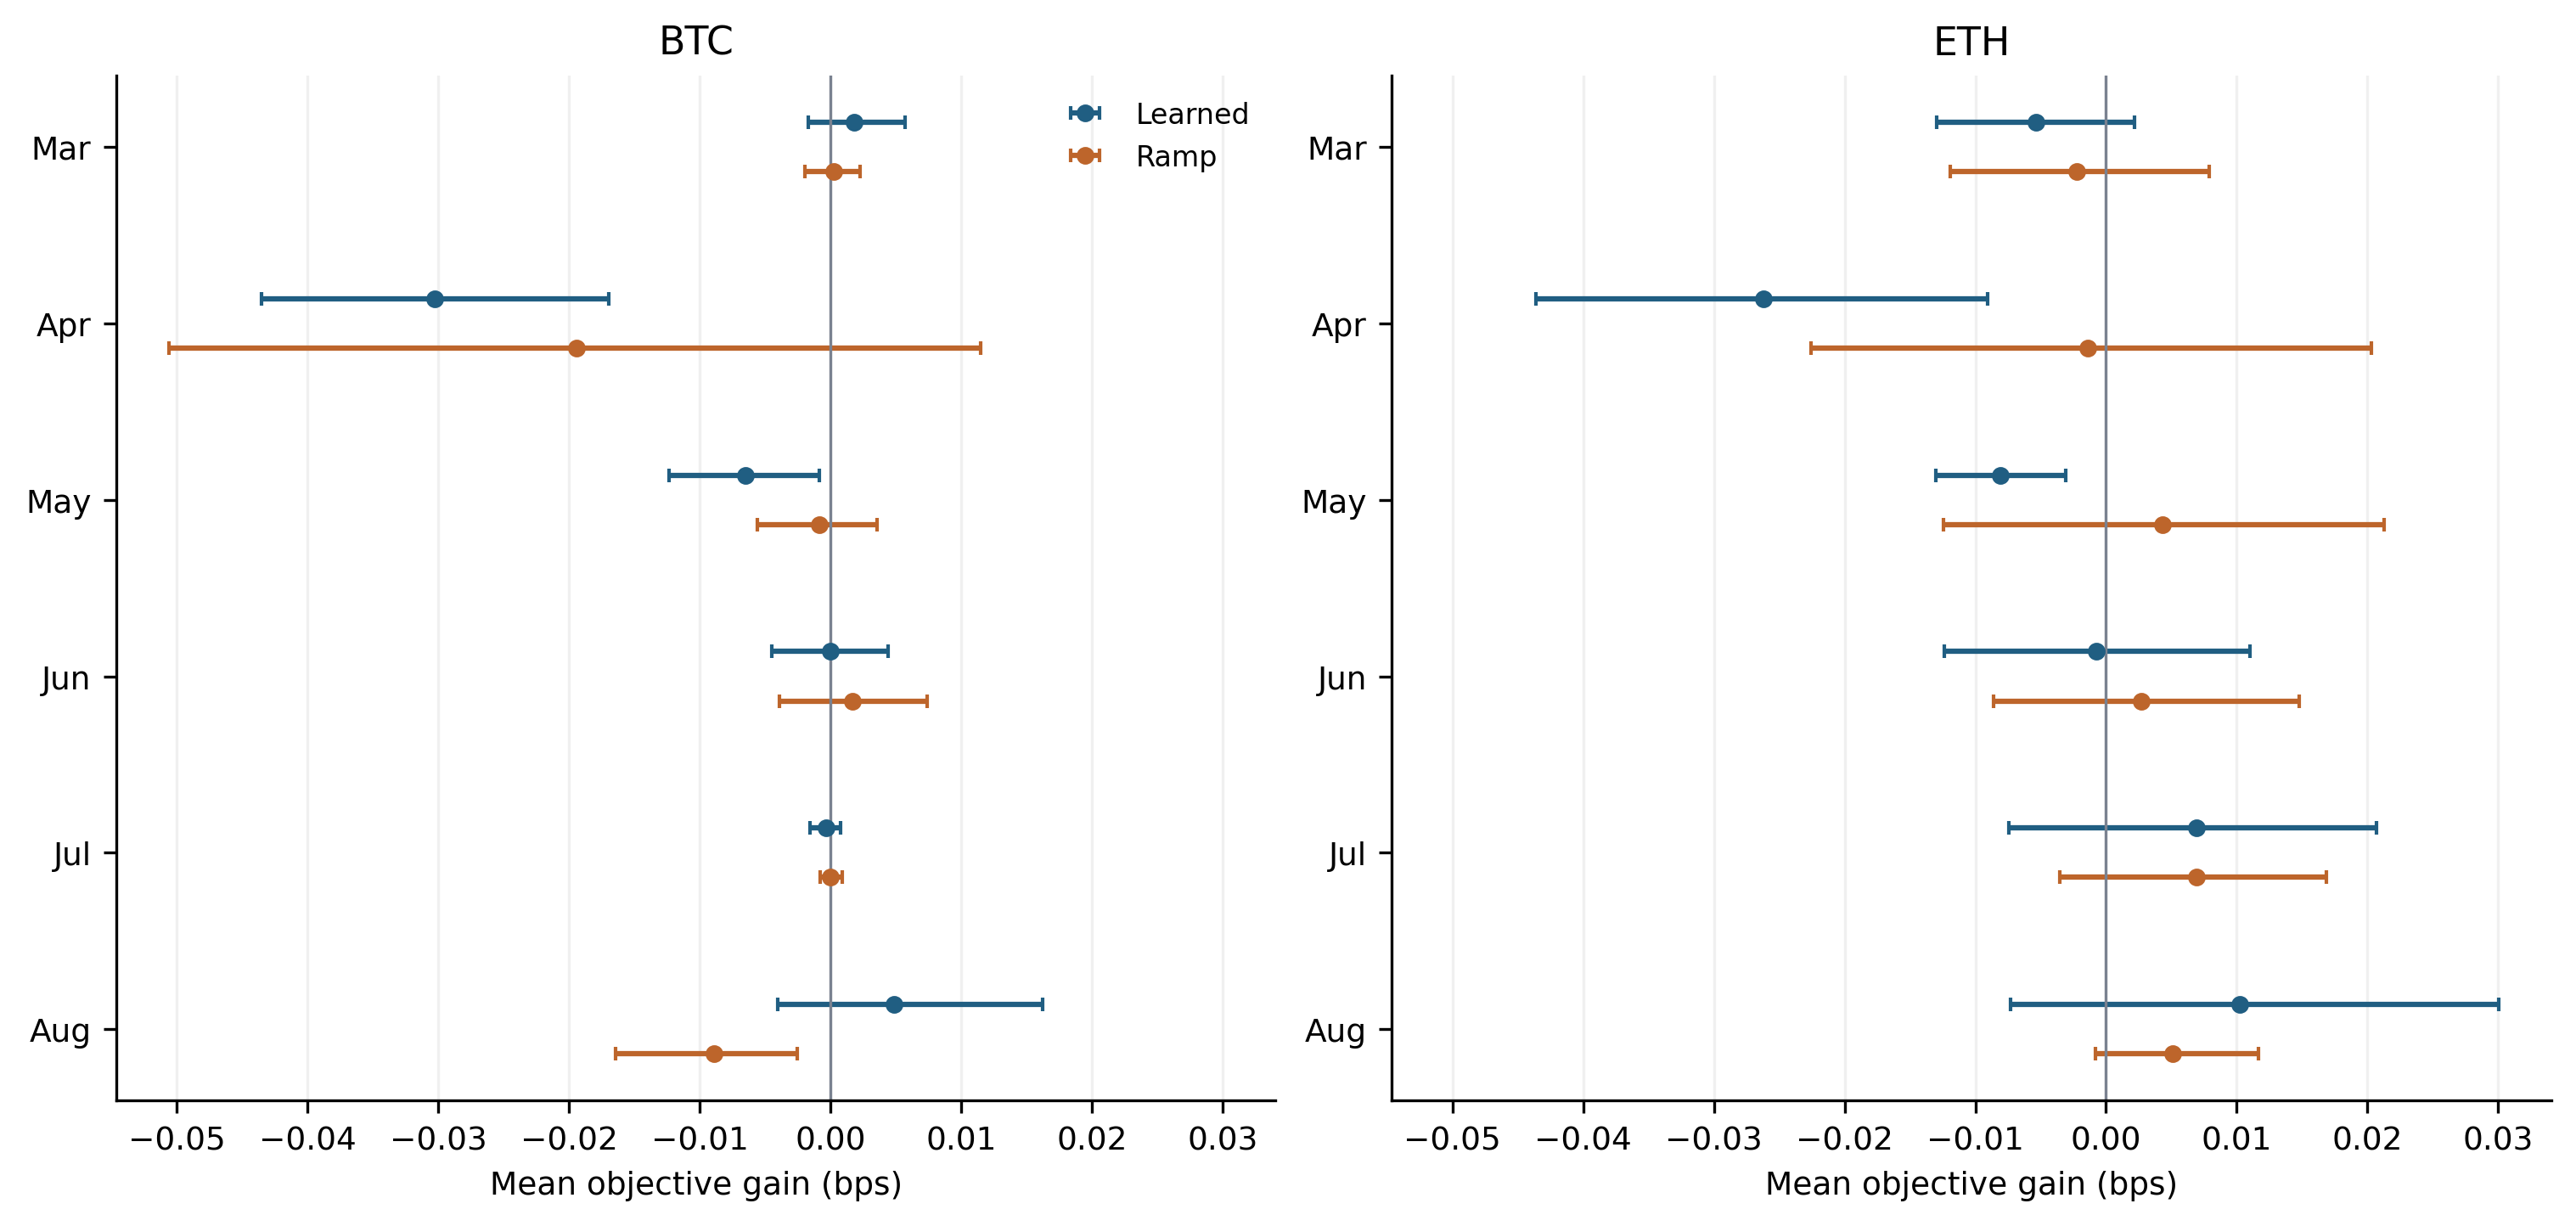
\includegraphics[width=\linewidth]{figures/fig04_monthly_gains.png}
\caption{All twelve primary asset--month evaluations. Learned and ramp points show full-exposure mean objective gains, with stored 95\% within-window calendar-day bootstrap intervals. Intervals condition on fitted forecasts, and overlapping windows are not independent replications.}
\label{fig:monthlygains}
\end{figure}

Figure~\ref{fig:monthlygains} shows the dispersion and within-window intervals. April contributes relatively large negative learned gains for both Bitcoin ($-0.03025$ basis points) and Ether ($-0.02624$). The final two Ether windows instead have positive gains of $0.00695$ and $0.01023$ basis points. Bitcoin's August learned gain is also positive, at $0.00488$ basis points. These changes indicate temporal heterogeneity in the relationship between fitted price profiles and realised timing payoffs. The design does not identify a causal market-regime explanation for that heterogeneity.

Endpoint diagnostics do not resolve the schedule comparison. Bitcoin in May records the highest reported hit rate, $52.6\%$, but its learned schedule loses $0.00648$ basis points against the baseline. Ether in May has positive terminal $R^2$ but a learned gain of $-0.00809$ basis points; its ramp gain is positive at $0.00434$. These are illustrative rows from the complete table, not selected tests of a general relationship between hit rates and gains. More decisively, each row's endpoint statistics are shared by the learned, ramp, mirror and parallel profiles despite their different decisions.

Equal weighting of the twelve asset--month means gives a learned gain of $-0.00446$ basis points, close to the episode-weighted $-0.00436$. Unequal month lengths therefore do not explain the pooled sign. Both summaries still describe overlapping rolling windows from one exchange and one eight-month input period; changing aggregation does not create independent evidence.

An additional ex post influence diagnostic recomputes the primary mean after omitting each evaluation month from both assets, without refitting forecasts or weights (Figure~\ref{fig:influence}). Omitting April changes the learned mean to $+0.00030$ basis points; all other single-month omissions retain a negative mean. The pooled negative sign is therefore sensitive to April's inclusion, despite its persistence across the specified cost grid. This display diagnoses concentration rather than defining a preferable subsample: the headline estimate retains every month, and no inferential interval is attached to the omission exercise.

\begin{figure}[htbp]\centering
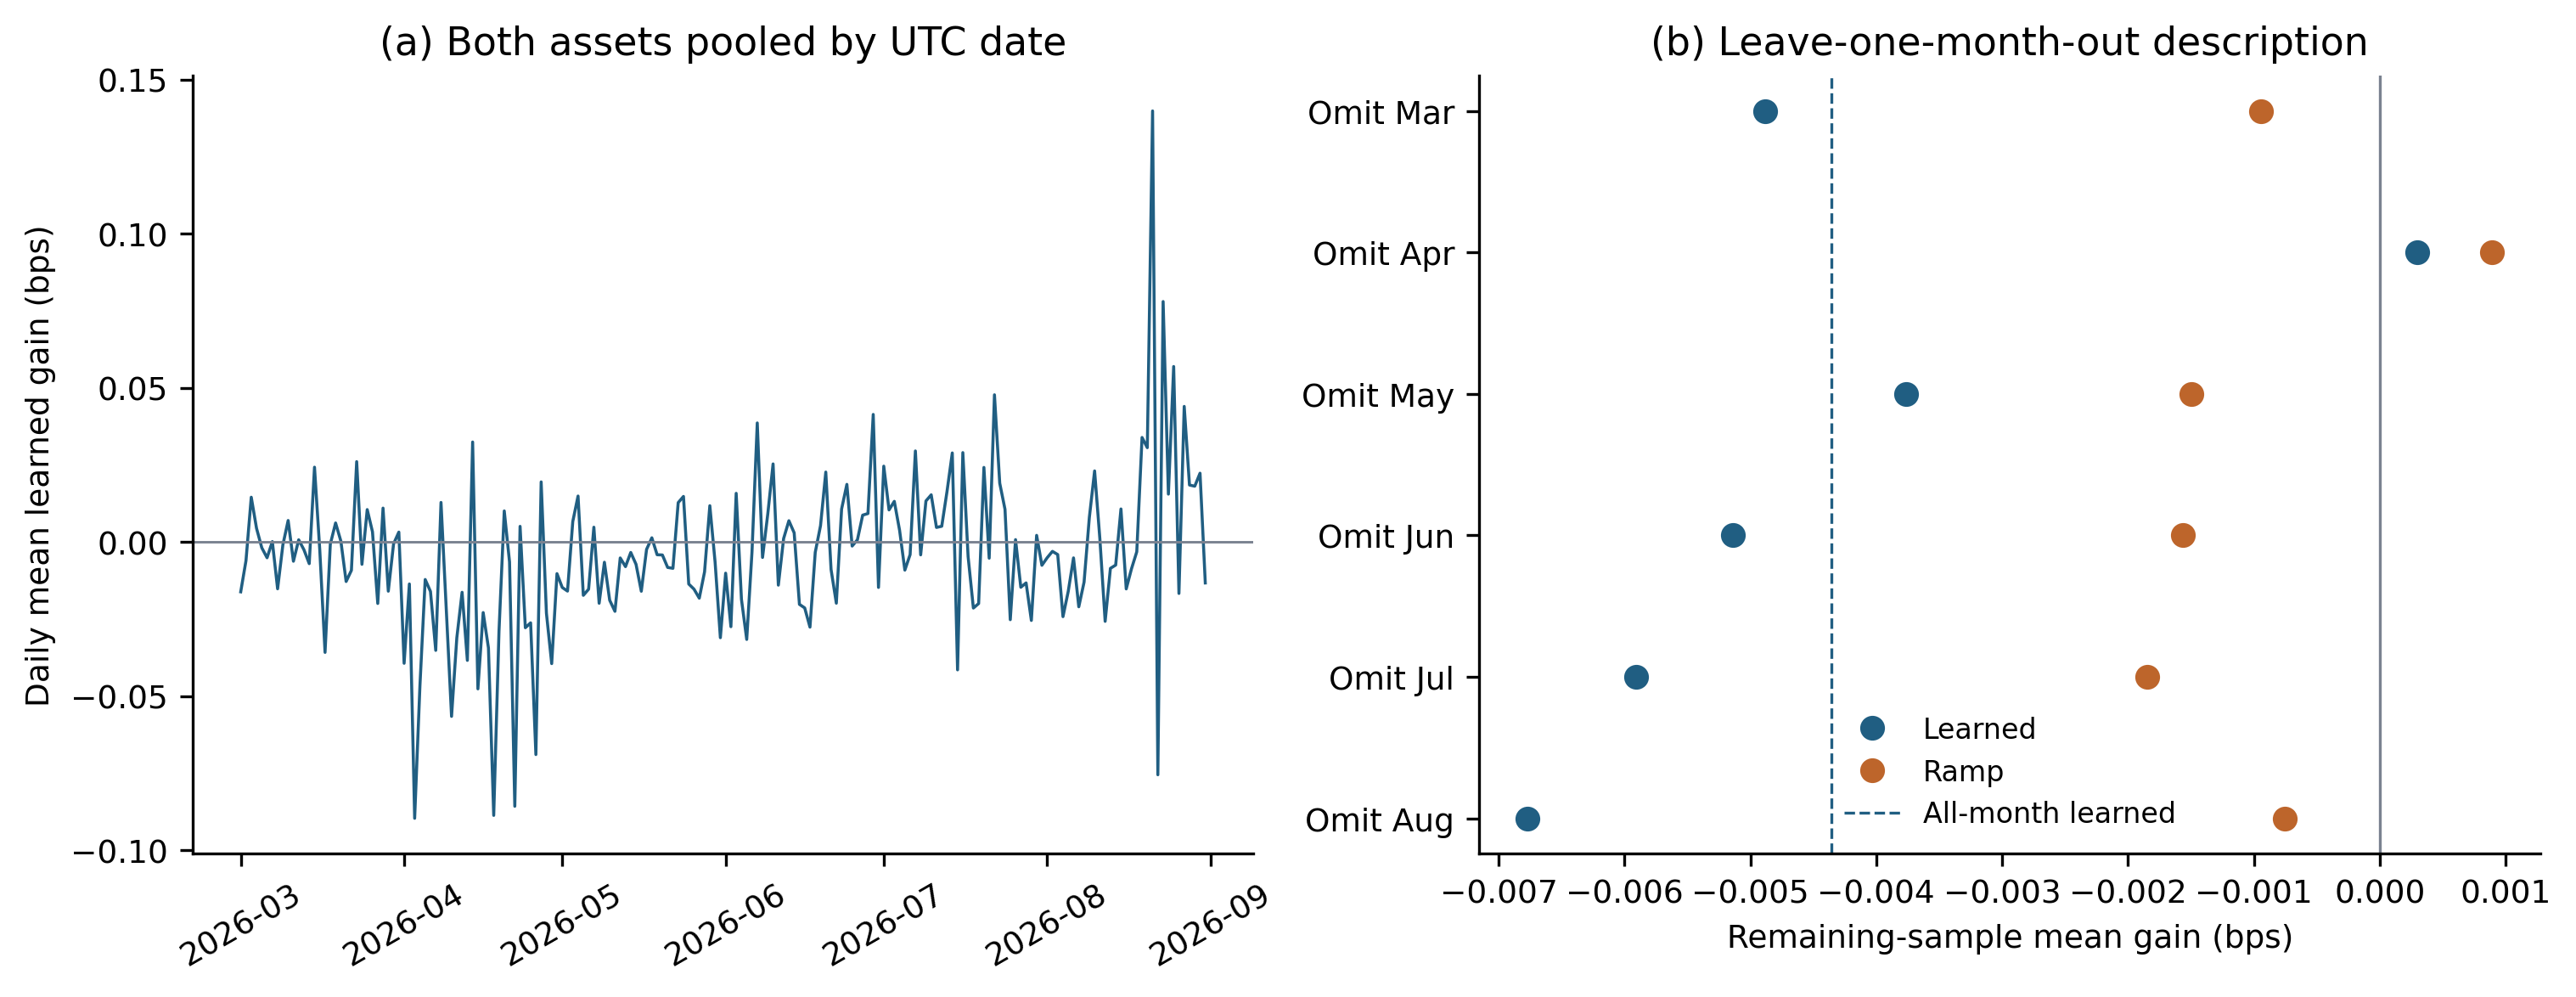
\includegraphics[width=\linewidth]{figures/fig08_descriptive_influence.png}
\caption{Additional ex post descriptive influence diagnostics from unchanged primary episodes. Panel (a) averages learned gains across both assets by UTC date. Panel (b) omits one evaluation month from both assets and recomputes the remaining mean; the dashed line is the full-sample mean. No forecasts or policies are refitted, and no confidence intervals or sample-selection recommendation are implied.}
\label{fig:influence}
\end{figure}

\subsection{Exposure fitting: partial improvement without a reliable advantage}
Table~\ref{tab:calibrated} compares ways of limiting the learned profile's influence. Half exposure yields mean objective gain $-0.00017$ basis points, with interval $[-0.00196,0.00171]$. Its movement towards zero follows the benefit--cost decomposition: halving exposure halves the linear timing term but quarters curvature cost. This improvement relative to full exposure is compatible with positive but weak timing information. It does not establish a positive expected execution saving.

\begin{table}[htbp]
\centering\small
\caption{Primary learned-profile exposure policies. Monetary gain drops the inventory-preference term when evaluating the same schedules. All gains are basis points; intervals refer to objective gain.}
\label{tab:calibrated}
\resizebox{\linewidth}{!}{\begin{tabular}{lrrr}
\toprule
Exposure policy & Objective gain & 95\% interval & Monetary gain \\
\midrule
Learned & -0.00436 & [-0.00829, -0.00047] & -0.00411 \\
Half learned & -0.00017 & [-0.00196, 0.00171] & -0.00007 \\
Plug-in & 0.00124 & [-0.00035, 0.00285] & 0.00125 \\
Lower-percentile & 0.00000 & [0.00000, 0.00000] & 0.00000 \\
\bottomrule
\end{tabular}
}
\end{table}

The plug-in rule selects positive weights in six of twelve windows and has pooled gain $0.00124$ basis points, interval $[-0.00035,0.00285]$. Its point estimate is favourable, but its conditional interval includes zero. The estimated weights vary markedly: Bitcoin's positive weights occur in May and July, while Ether's occur in April and June--August. Prior-month fitting therefore sometimes retains forecast exposure and sometimes rejects it. The data do not demonstrate a stable gain from this policy across future periods.

\begin{figure}[htbp]\centering
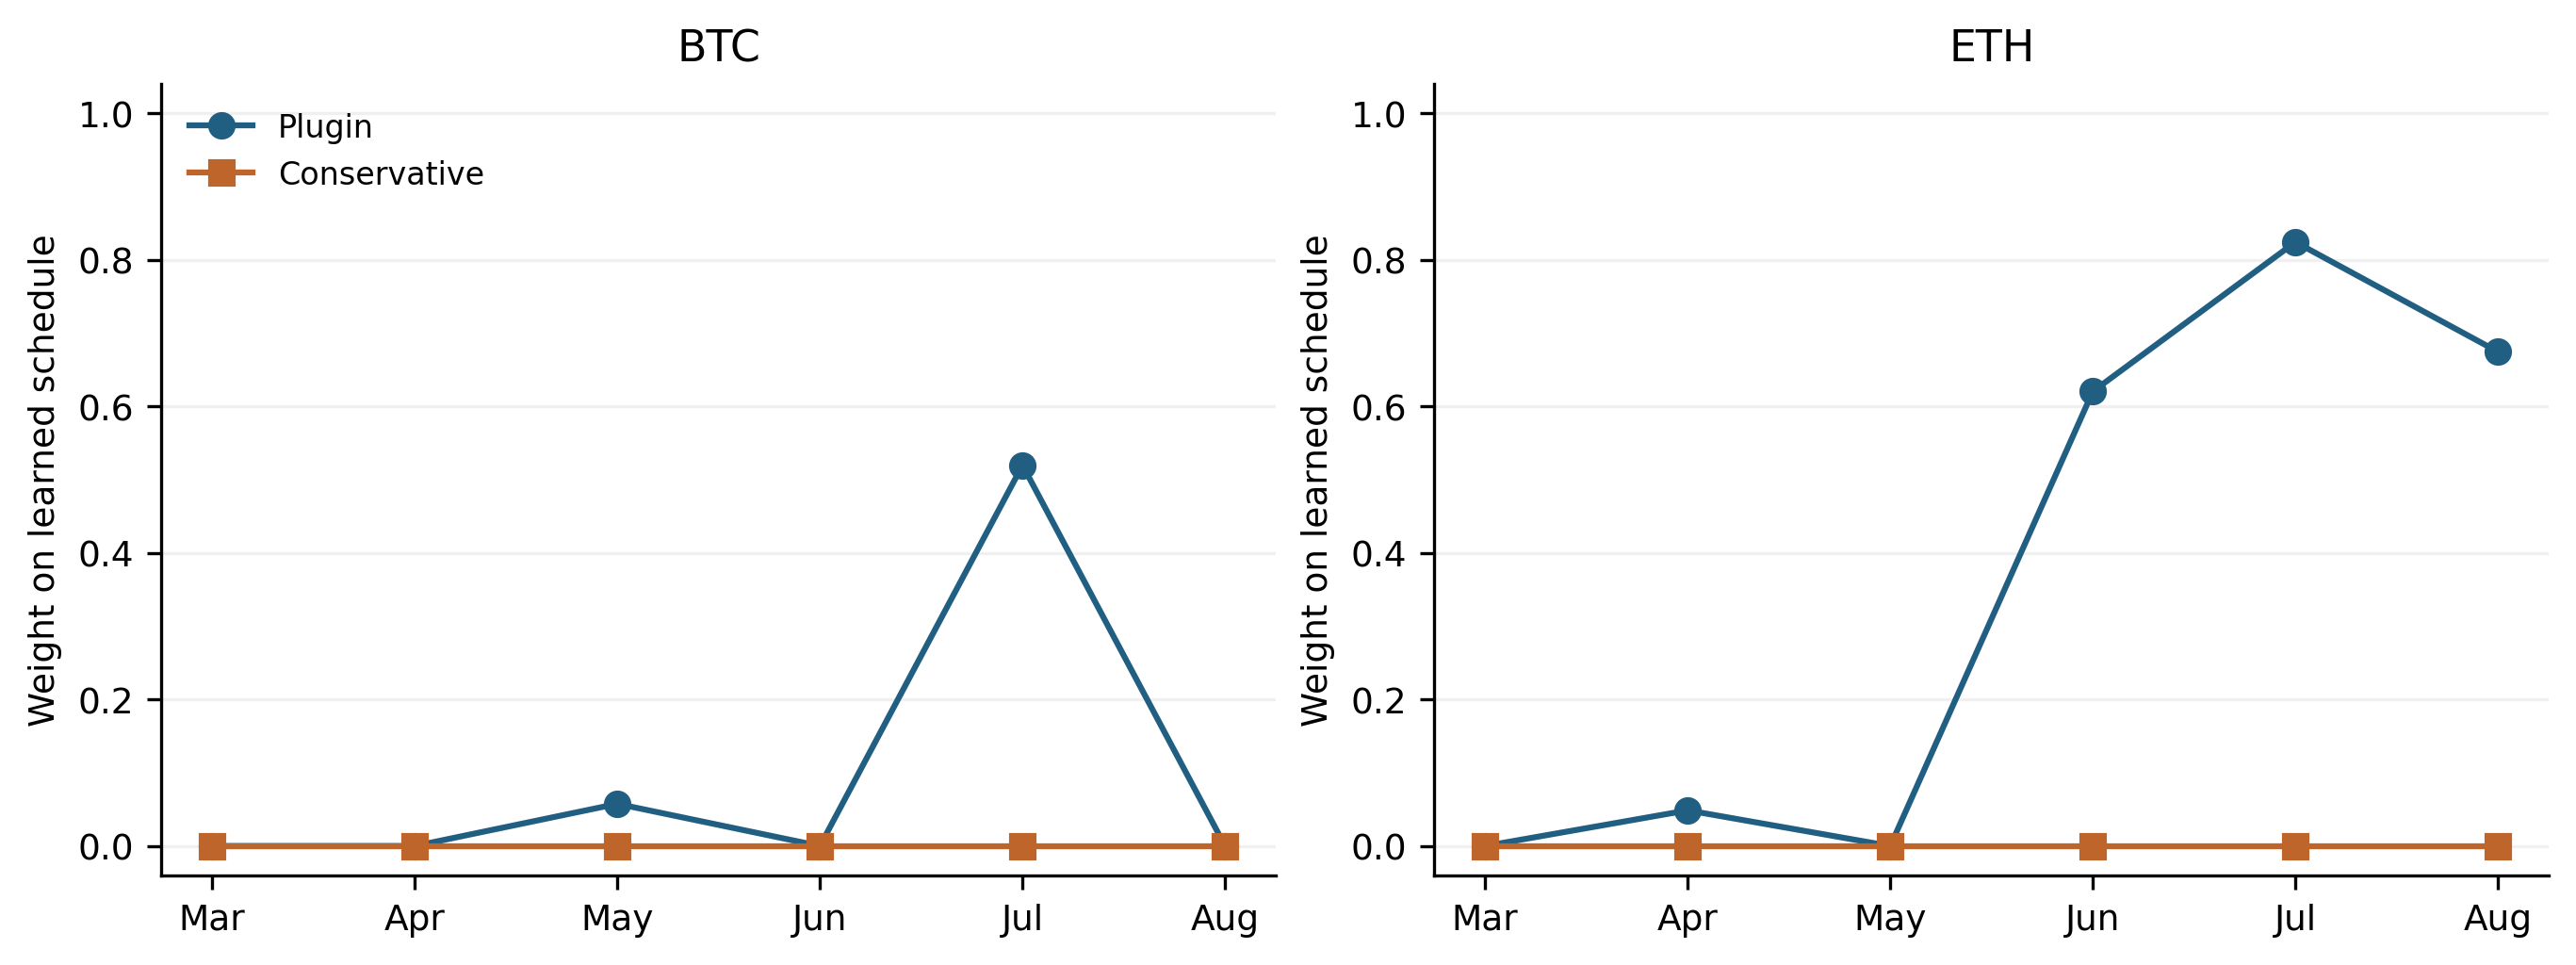
\includegraphics[width=\linewidth]{figures/fig05_calibrated_exposure.png}
\caption{Primary schedule-mixture weights fitted on the preceding calibration month. Plug-in weights are positive in six windows; lower-percentile weights are zero throughout. These weights are determined before each evaluation month within the retrospective design.}
\label{fig:exposure}
\end{figure}

Figure~\ref{fig:exposure} makes the variation in fitted exposure explicit. The lower-percentile rule selects zero in every window. Its realised paired gains are identically zero because its schedule equals the baseline, so its degenerate interval expresses policy identity. It does not imply certainty about future market conditions or the baseline's own costs. In this sample, the rule avoids the full-exposure loss, but it contributes no action beyond unconditional abstention. Accordingly, this result cannot establish superior calibration, robustness or safety.

Evaluating the pooled quadratic curve after observing all outcomes helps interpret these comparisons. Positive linear benefit creates a region in which smaller exposure has a positive retrospective mean gain; curvature eventually dominates as exposure increases. Any maximum computed from that evaluation curve is hindsight information. It is distinct from the monthly weights fitted on preceding data and is not reported as an implementable additional policy.

\subsection{Sensitivity to assumed impact and inventory preferences}
Full learned exposure has a negative pooled point estimate under every specified cost scenario (Table~\ref{tab:sensitivity}). At $\eta=0.5,r=0$, the estimate is $-0.01420$ basis points and its interval includes zero. Adding the inventory preference at the same impact coefficient gives $-0.01562$. At $\eta=5$, the losses are smaller, approximately $-0.00171$ and $-0.00172$ for $r=0$ and $r=1$. The remaining intervals exclude zero under the stated conditional resampling procedure.

\begin{table}[htbp]
\centering\small
\caption{All six hypothetical cost specifications. The same observations underlie each scenario, so these are sensitivity comparisons rather than independent replications. Full policy results are retained in the machine-readable output.}
\label{tab:sensitivity}
\resizebox{\linewidth}{!}{\begin{tabular}{rrrrr}
\toprule
$\eta$ & $r$ & Learned gain & 95\% interval & Plug-in gain \\
\midrule
0.5 & 0 & -0.01420 & [-0.02929, 0.00141] & 0.00533 \\
0.5 & 1 & -0.01562 & [-0.02908, -0.00193] & 0.00409 \\
2 & 0 & -0.00427 & [-0.00833, -0.00024] & 0.00133 \\
2 & 1 & -0.00436 & [-0.00829, -0.00047] & 0.00124 \\
5 & 0 & -0.00171 & [-0.00333, -0.00010] & 0.00053 \\
5 & 1 & -0.00172 & [-0.00333, -0.00014] & 0.00052 \\
\bottomrule
\end{tabular}
}
\end{table}

\begin{figure}[htbp]\centering
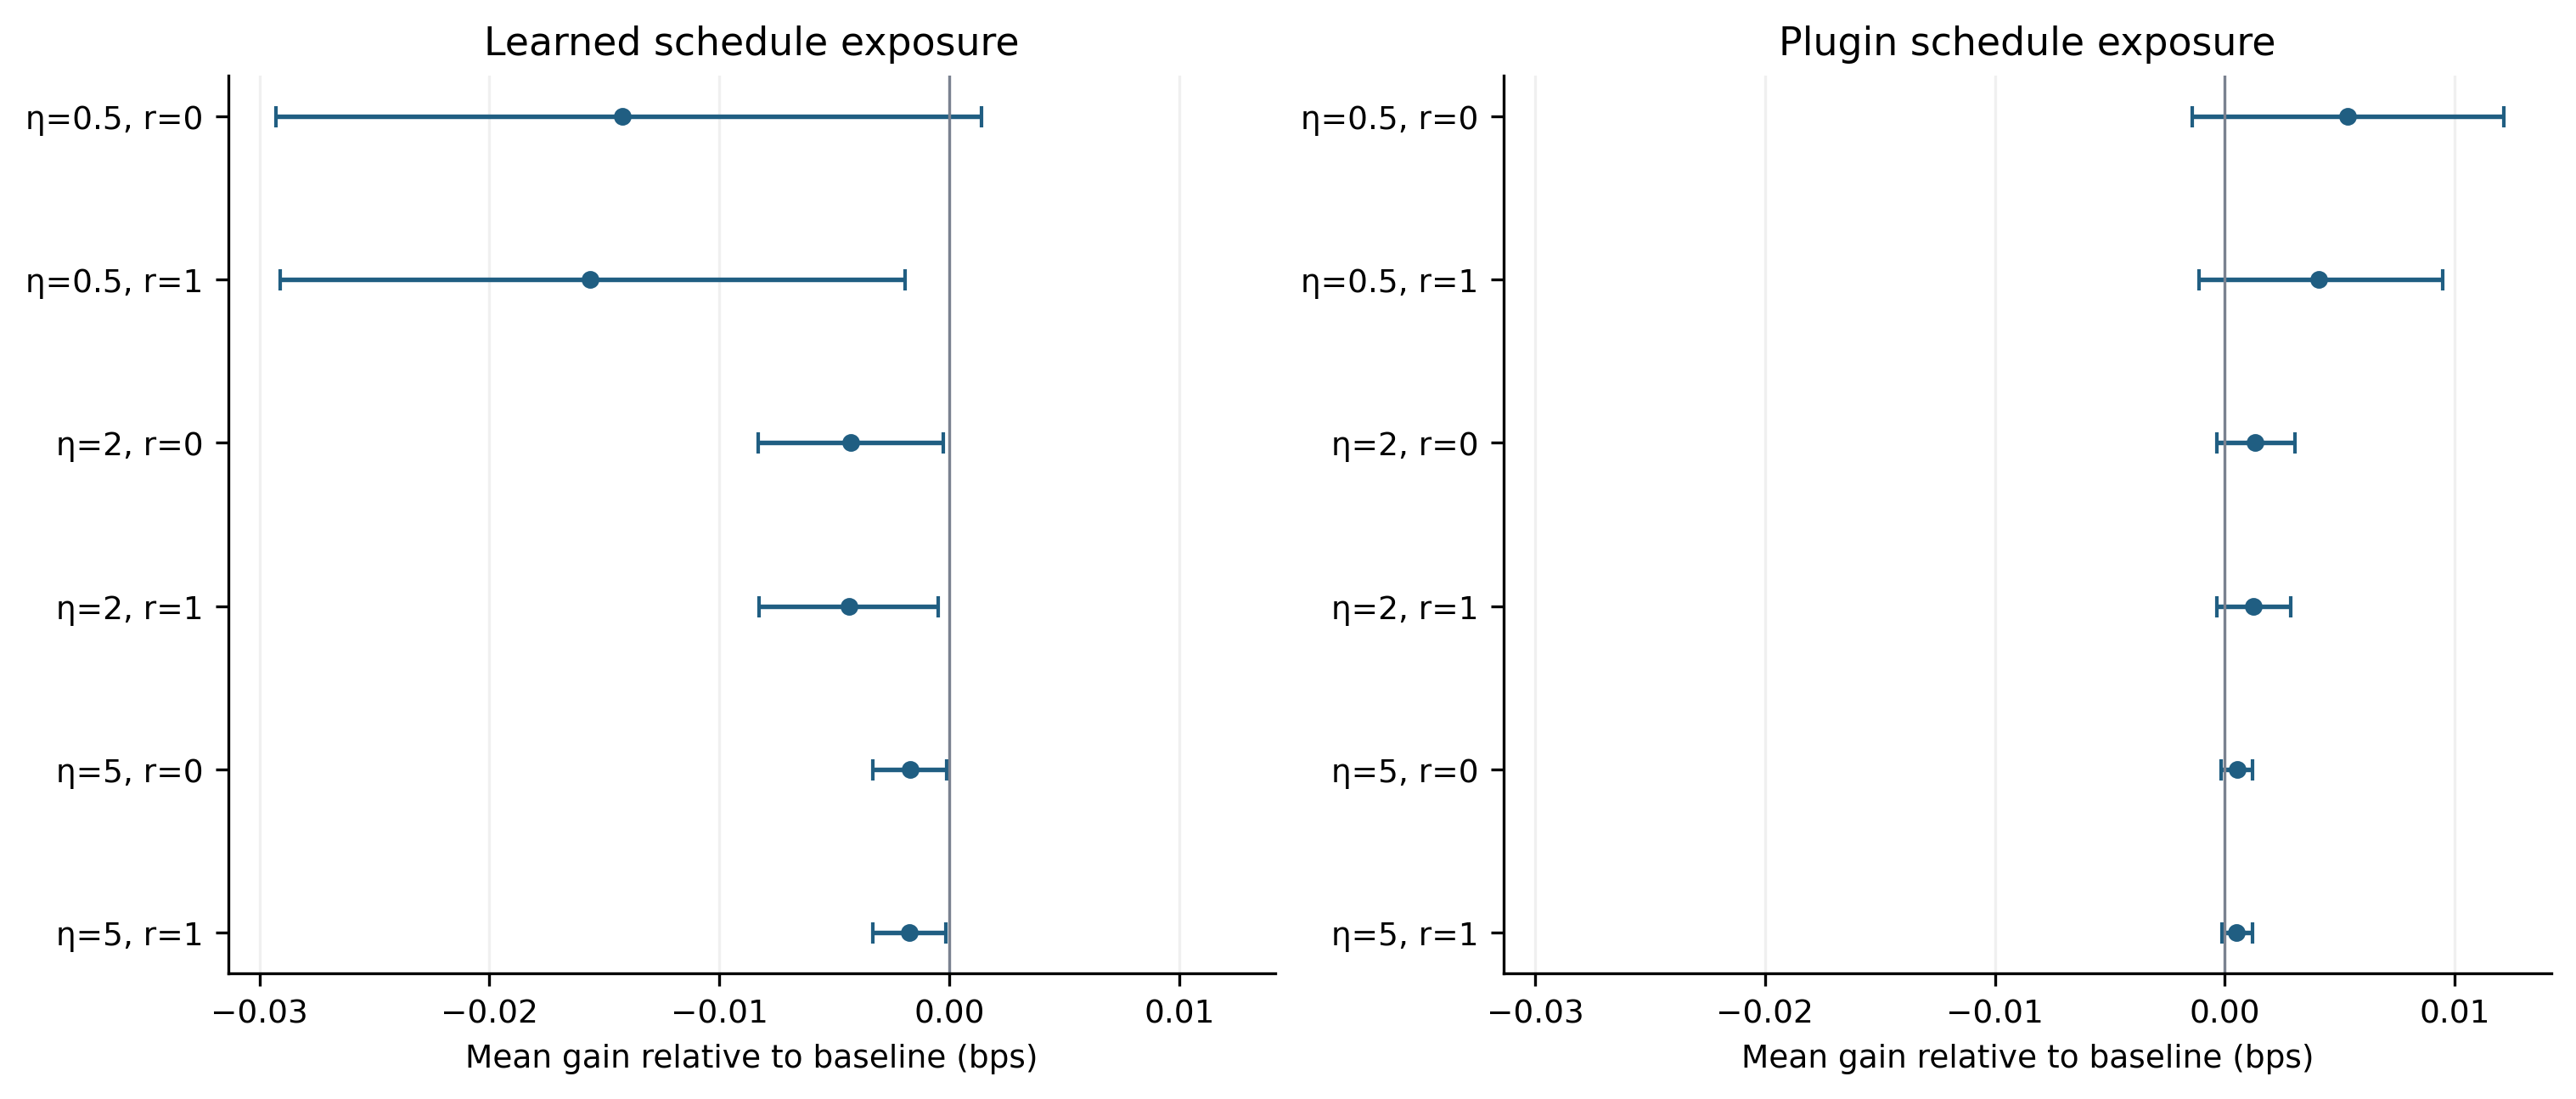
\includegraphics[width=\linewidth]{figures/fig07_cost_sensitivity.png}
\caption{All six specified cost scenarios for full learned exposure and the prior-month plug-in mixture. Points and conditional 95\% day-bootstrap intervals come from the unchanged analysis. Impact and inventory coefficients are assumed rather than estimated from exchange execution.}
\label{fig:sensitivity}
\end{figure}

Figure~\ref{fig:sensitivity} also displays plug-in intervals across the full cost grid. Increasing the impact coefficient changes the optimised schedule itself. Larger penalties discourage reallocation, so the smaller loss at high $\eta$ is not evidence that greater real-world trading costs improve an unchanged strategy. It reflects the response of a cost-aware optimiser to a stronger assumed penalty. The six-scenario grid demonstrates persistence of the negative full-exposure point estimate over this specified range; it cannot validate the coefficients as plausible costs for a particular parent-order size.

\begin{figure}[htbp]\centering
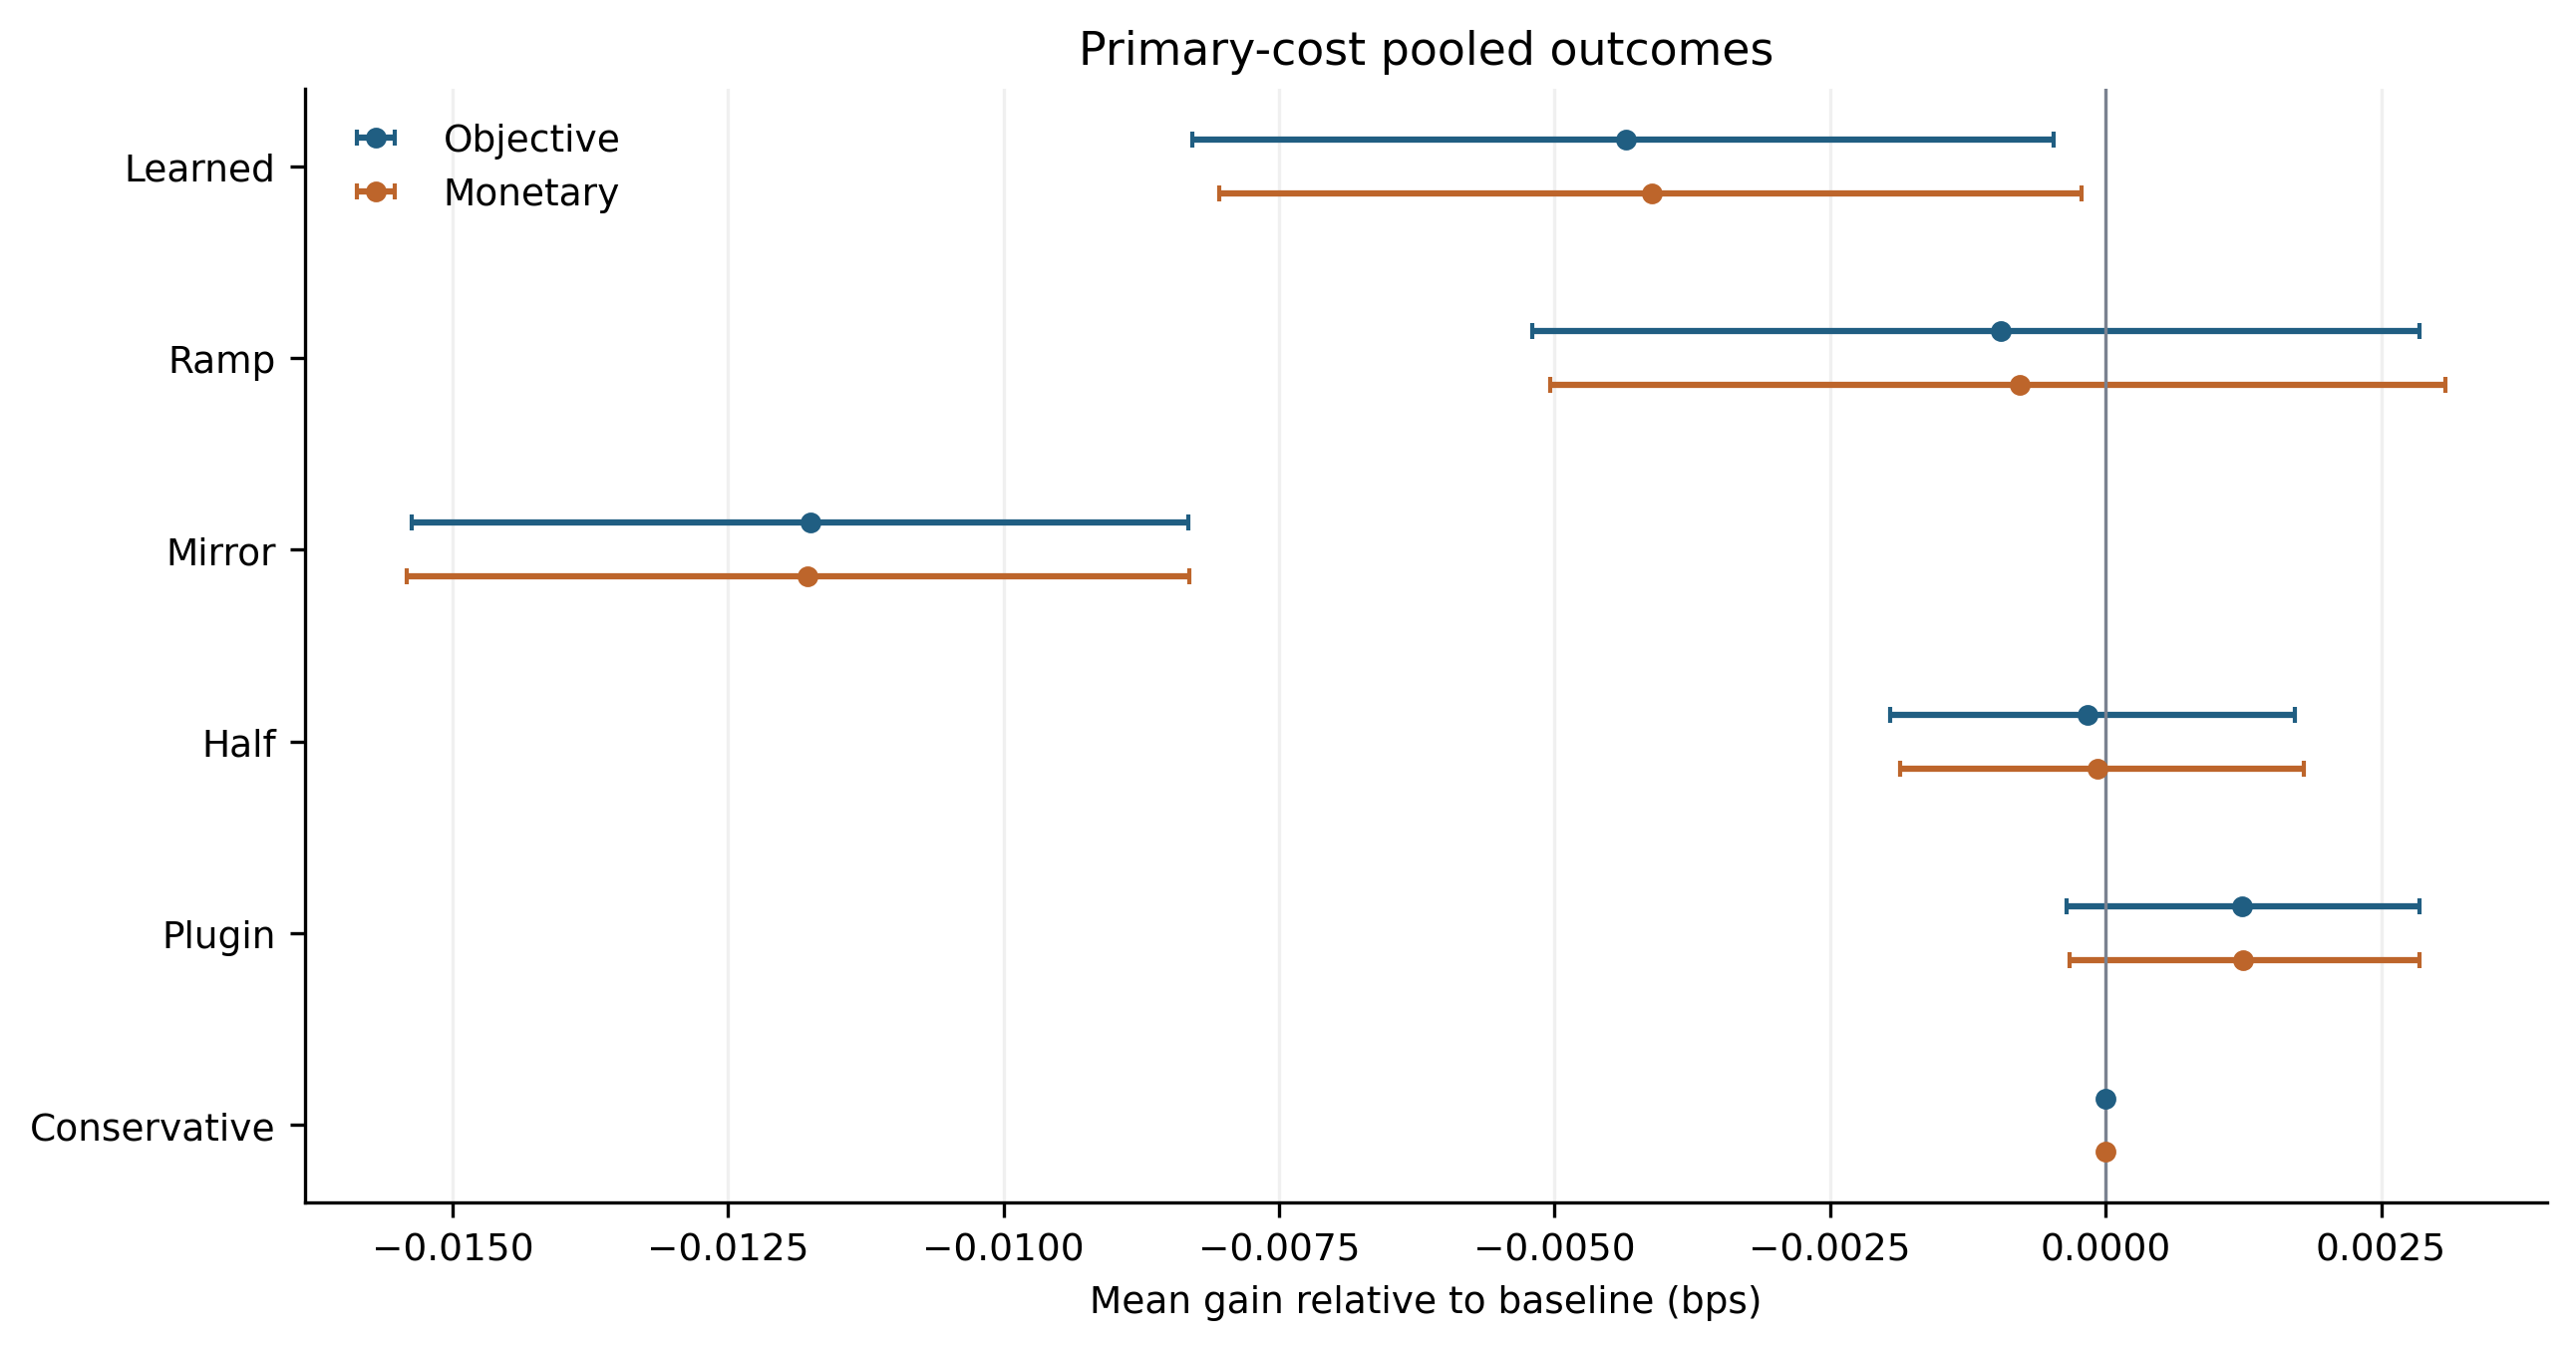
\includegraphics[width=\linewidth]{figures/fig06_objective_monetary.png}
\caption{Primary objective and monetary gains with conditional 95\% day-bootstrap intervals. Monetary scoring removes the inventory preference from the same schedules, while retaining hypothetical impact charges. These are replay outcomes, not observed trading profits.}
\label{fig:monetary}
\end{figure}

Figure~\ref{fig:monetary} separates the two scoring conventions. The inventory term also requires a separate interpretation. At the primary setting, full-exposure monetary gain is $-0.00411$ basis points, compared with objective gain $-0.00436$. Thus the negative conclusion is not generated solely by including a noncash inventory preference. Plug-in monetary gain is $0.00125$ basis points, close to its objective gain. Both monetary measures still contain hypothetical impact charges and minute-open price proxies. Removing the inventory term does not transform them into observed cash savings.

\subsection{Economic interpretation and scope}
The findings support a practical evaluation sequence: distinguish endpoint prediction from temporal price contrasts, examine the schedule induced by those contrasts, and compare its gross timing benefit with the cost of taking that action. This sequence is useful even when the final empirical conclusion is negative. Here endpoint scores cannot distinguish the constructed policies, average learned timing alignment is positive, and full exposure nevertheless reduces the model objective's performance. These are different propositions, each requiring its own evidence.

The present replay cannot establish executable trading gains or a crypto-specific structural mechanism. It lacks parent-order size, quoted spreads, depth, queue position, fill uncertainty and endogenous impact. Bar opens do not verify fills, and an order large enough to change prices would challenge the assumed common realised path. Conversely, an economically richer execution setting might change both relative costs and the appropriate forecast target. The contribution that carries beyond this illustration is the matched-endpoint comparison and benefit--cost accounting, while its quantitative performance conclusions remain conditional on the specified data, schedules and hypothetical costs.
